% \documentclass{article}
\documentclass[11pt]{article}
\oddsidemargin 0.0in \evensidemargin 0.0in
\topmargin 0in
\usepackage{amsmath}
\usepackage{amssymb}
\usepackage[utf8]{inputenc}
%\usepackage[pdftex]{graphicx,color}
\usepackage{graphicx}
%\usepackage{color}
%\usepackage{epsfig}

\usepackage{algorithm}
\usepackage{algorithmic}
\usepackage{caption}
\usepackage{latexsym}
\usepackage{amsfonts}
\usepackage{amstext}
\usepackage{amsthm}
\usepackage{url}

\usepackage{enumerate}

\usepackage{color}

\usepackage{pdfpages}

\usepackage{tikz}

%-----------------------------------
% Disables algorithm captions
\DeclareCaptionLabelFormat{numberless}{\textbf{#1}}
\captionsetup[algorithm]{labelformat=numberless}
%-----------------------------------

\textwidth 6in \textheight 8in
\newtheorem{theorem}{Theorem}
\newtheorem{lemma}[theorem]{Lemma}
\newtheorem{claim}[theorem]{Claim}
\newtheorem{prop}[theorem]{Proposition}
\newtheorem{remark}[theorem]{Remark}
\newtheorem{definition}[theorem]{Definition}
\newtheorem{corollary}[theorem]{Corollary}
\newtheorem{observation}[theorem]{Observation}
\newtheorem{invariant}[theorem]{Invariant}
\newtheorem{procedure}[theorem]{Procedure}
\newtheorem{property}[theorem]{Property}
\newtheorem{fact}[theorem]{Fact}
\newtheorem{question}{Question}
\newtheorem{assertion}[theorem]{Assertion}
\newtheorem{example}[theorem]{Example}

%-----------------------------------


\begin{document}

% Compilation of common latex templates I end up using in my homework

\title{Homework XXX, Solution Set}
\author{Keyur Panchal\\keyur.panchal@nyu.edu}
% \email{keyur.panchal@gmail.com}
\date{\today}

\maketitle

\tableofcontents
\section{Templates}

\subsection{Answer format}
\bigskip \noindent 1. \textbf{Answer:}

\bigskip \noindent 2. \textbf{Answer:}

\bigskip \noindent 3. \textbf{Answer:}

\bigskip \noindent 4. \textbf{Answer:}

\pagebreak

% templates
\subsection{Pseudocode}
\begin{algorithm}
	\texttt{Input: A: xx B: yy n: count. }
	\begin{algorithmic}
    	\caption{Algorithm$(A, B, n-1)$}
	    \IF{n=1}
    	    \STATE
	    \ELSE 
	    \STATE Algo$(A, B, n-1)$
	    \ENDIF
            \FOR{$r = 0 \to n$}
                    \FOR{$i = 1 \to n-r$}
                        \STATE Len $=$ L[$i+r$] $-$ L[$i-1$]
                    \ENDFOR
            \ENDFOR
	\end{algorithmic}
\end{algorithm}

\subsection{Lists}

\begin{enumerate}
    \item {numbered list}
\end{enumerate}

\begin{itemize}
    \item {unordered list}
\end{itemize}

\subsection{Table}
\begin{center}
\begin{tabular}{ c c c }
 Size of subproblems & Number of subproblems & Non-recursive cost\\ 
 $n = 2^k$ & $1$ & $\log n = k$ \\
\end{tabular}
\end{center}

\subsection{Multi-line aligned equations}

\begin{align*}
T(n) &= k + (k-1) + (k-2) + ... + 2 + 1 \\
&= \frac{k(k+1)}{2} \\
\end{align*}

\subsection{Equation spanning multiple lines}

\[
\text{MinEdit}(n, m, k) = \begin{cases}
\mbox{$m$,} & \mbox{if $n = 0$} \\ \mbox{$n$,} & \mbox{if $m = 0$} \\ \mbox{$\min{\bigg\{\max\log\bigg\}}$,} & \mbox{if $|n - m | < k \text{ and } u_n \neq v_m$}
\end{cases}
\]


\subsection{Tree drawing}
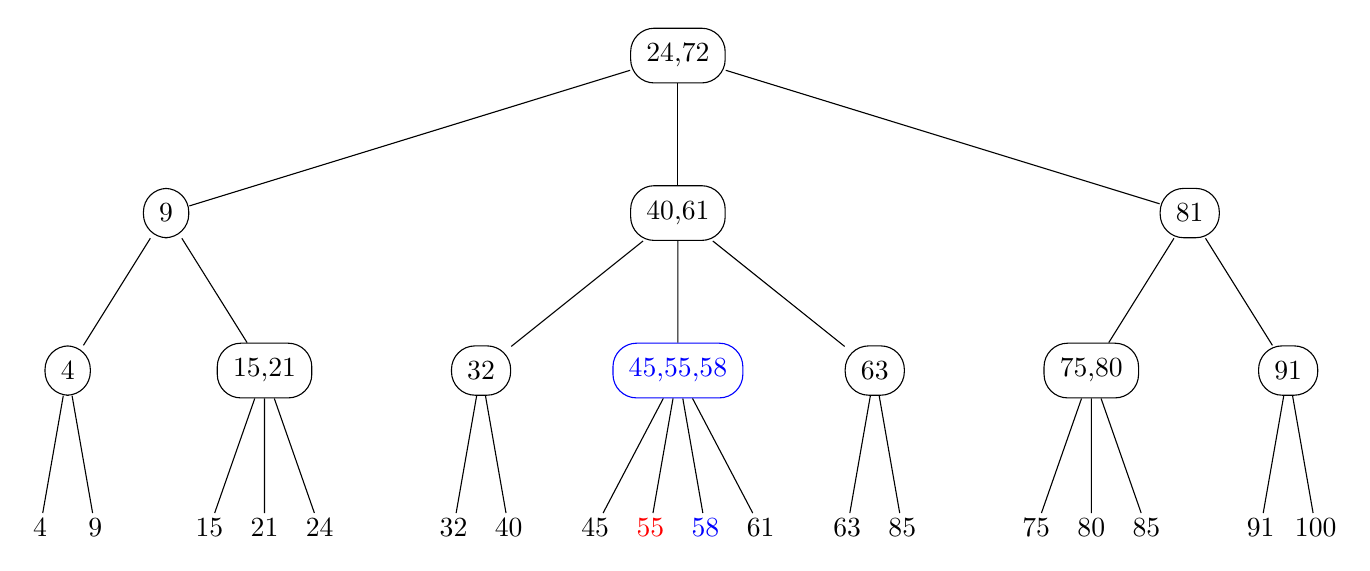
\begin{tikzpicture}
\tikzstyle{internal}=[draw,rectangle,rounded corners=3mm,inner sep=2mm,minimum size=2mm]
\tikzstyle{leaf}=[draw=none,inner sep=2, minimum size=2mm]
\node[internal] {24,72}
    [grow=down,sibling distance=65mm,level distance=20mm]
    child {node [internal]{9}
    [sibling distance=25mm]
        child {node [internal]{4}
        [sibling distance=7mm]
            child {node [leaf] {4}}
            child {node [leaf] {9}}
        }
        child {node [internal]{15,21}
        [sibling distance=7mm]
            child {node [leaf] {15}}
            child {node [leaf] {21}}
            child {node [leaf] {24}}
        }
    }
    child {node [internal]{40,61}
    [sibling distance=25mm]
        child {node [internal]{32}
        [sibling distance=7mm]
            child {node [leaf] {32}}
            child {node [leaf] {40}}
        }
        child {node [internal,color=blue]{45,55,58}
        [sibling distance=7mm]
            child {node [leaf] {45}}
            child {node [leaf,color=red] {55}}
            child {node [leaf,color=blue] {58}}
            child {node [leaf] {61}}
        }
        child {node [internal]{63}
        [sibling distance=7mm]
            child {node [leaf] {63}}
            child {node [leaf] {85}}
        }
    }
    child {node [internal]{81}
        [sibling distance=25mm]
        child {node [internal]{75,80}
        [sibling distance=7mm]
            child {node [leaf] {75}}
            child {node [leaf] {80}}
            child {node [leaf] {85}}
        }
        child {node [internal]{91}
        [sibling distance=7mm]
            child {node [leaf] {91}}
            child {node [leaf] {100}}
        }
    };
\end{tikzpicture}

\end{document}